\PassOptionsToPackage{table}{xcolor}
\documentclass{article}
% \documentclass{report}
\usepackage[utf8]{inputenc}
\usepackage{xspace}
\usepackage{url}
\usepackage{hyperref}
\usepackage{fancyhdr}
\usepackage{cite}
\usepackage{pgfgantt}
\usepackage{todonotes}
\usepackage[icelandic,UKenglish]{babel}
\usepackage[UKenglish]{datetime}
\usepackage[T1]{fontenc}
\usepackage{graphicx}
\usepackage[table]{xcolor}
\usepackage{enumitem}% http://ctan.org/pkg/enumitem
\usepackage[gen]{eurosym}
\usepackage{multicol}
\graphicspath{ {./images/} }
\usepackage[titletoc,title]{appendix}
\usepackage{pdfpages}

\fancypagestyle{plain}{ %
  \fancyhf{} % remove everything
  \renewcommand{\headrulewidth}{0pt} % remove lines as well
  \renewcommand{\footrulewidth}{0pt}
}
% \setlength{\topskip}{0mm}
\setlength{\headheight}{15pt}
% \setlength{\topmargin}{-5.4mm}
% \setlength{\textheight}{230mm}
\setlength{\textwidth}{180mm}
\setlength{\oddsidemargin}{-5.0mm}
% \setlength{\evensidemargin}{10.0mm}
% \setlength{\captionmargin}{7mm}

% \newcounter{sectocnonumdepth}
% \setcounter{sectocnonumdepth}{0}

\newcommand{\dell}{Dellingr\xspace}
\newcommand{\einfra}{e-infrastructure\xspace}
\newcommand{\Lin}{LINPACK\xspace}
\newcommand\EatDot[1]{}
\newcommand{\np}{national provider\xspace}
\newcommand{\nps}{\np{s}\xspace}
\newcommand{\coreh}{core-hours\xspace}
\newcommand{\HLT}{High-Level track\xspace}
\newcommand{\pilot}{first test of a Nordic resource-sharing framework\xspace}

\begin{document}

\begin{center}

\includegraphics[width=\textwidth]{neic_logo_large.png}
\end{center}

\vspace{0.5in}
{\Huge  \dell Final Report} \hrule
\vspace{0.5in}

\noindent
{\large

{The report is drawn-up in agreement between NeIC as the project owner represented by Tomasz Malkiewicz and the project manager John White. 
It is verified through a Steering Group decision.
}
}

\begin{center}
% \rowcolors{2}{gray!25}{white}
\rowcolors{2}{white}{gray!25}
\begin{tabular}{|l| l| l| l|} \hline

& Name
& Partner/Activity
& Date \\ \hline
From & 
John White &
NeIC & 
2020/04/15 \\ \hline
Reviewed by &
Tomasz Malkiewicz & 
NeIC & 
\\ \hline
Approved by &
 & 
 & 
\\ \hline
\end{tabular}
\end{center}

{\bf \large Edition history:}

\begin{center}
\rowcolors{2}{gray!25}{white}
\begin{tabular}{|l| l| l| l|} \hline
Issue
& Date
& Comment
& Author/Partner \\ \hline
From & 
John White &
 v1 & 
 NeIC \\ \hline
Reviewed by &
Tomasz Malkiewicz & 
& 
NeIC \\ \hline
Approved by &
 & 
 & 
\\ \hline
\end{tabular}
\end{center}

{\bf \large Abstract:}
\noindent
{The report summarizes the achievements of the \dell project in relation to the objective. Also  experiences and recommendations for improving working methods for future projects are given.}

\begin{center}
\rowcolors{2}{gray!25}{white}
\begin{tabular}{|l| l| l|} \hline
\multicolumn{3}{|c|}{\bf Comprehensive information about the project} \\ \hline
\bf Type of Project: & \multicolumn{2}{|c|}{Collaboration project} \\ \hline
\bf Scope & \bf Result & 0.6 \\ \cline{2-3}
      & \bf Time & 0.3 \\ \cline{2-3}
      & \bf Cost & 0.1 \\ \hline
\bf Documentation & \multicolumn{2}{|l|}{\bf Internal: {\url{https://wiki.neic.no/int/Dellingr}}} \\
\bf Location & 
\multicolumn{2}{|l|}
{\bf External: {\url{https://wiki.neic.no/wiki/Dellingr
}}} \\ \hline
\end{tabular}
\end{center}
% {\it Specify the type of project (prestudy, development project, delivery project, etc.). Describe the scope of the project in the form of the result (what has been delivered), the duration of the project, and also the total cost. Also specify where the project documentation is stored.}

\newpage
\tableofcontents
\newpage

\section{Basic Information}

\subsection{The project}
% {\it Briefly describe the project background, possibly also its history. Also specify if it is an individual project, part of a NeIC strategic area or related to other projects. Describe cooperation with the national e-infrastructure providers. If applicable, also describe interactions with other stakeholders of NeIC; research communities, researchers, etc}

The \dell project was instigated by the NeIC board in 2014 based on the observation that researchers are increasingly using sophisticated computational and data analysis systems to address research problems.

As a result, research collaborations are evolving and expanding to include the wider range of fields and domains necessary to consider these problems at different scales, with more integrated approaches and in larger scientific and societal contexts. Consequently, long-term access to well supported computational and associated data analysis systems is fundamental to the success of the research endeavours. However, the sophistication of the systems has moved in new directions with the growth (and divergence) of High Performance Computing (HPC), cloud computing, data intensive computing as well as citizen science. The increasing sophistication of systems bring out additional considerations in terms of costs, time frames and user support.

The exploration of a coordinated long term Nordic \einfra approach that makes computational, data and user support readily available to all Nordic researchers in all fields reflects the growing reality for research projects in the context of international collaborations, programs, and international competition.
An effort focused on HPC and related aspects complements these efforts and is consistent with strategic directions in the Nordic region as embodied in the Nordic e-Science Action Plan:
\begin{itemize}
\item Action 6: Nordic Sharing and Exchange of \einfra Resources
\item Action 8: Nordic High Performance Computing Collaboration.
\end{itemize}

This is also embodied in the NeIC Strategy Implementation Plan 2016-2020, which has Share Resources as one of the four focus areas.
\einfra resources can be hardware (CPU cycles, storage), software, services, or human resources. 

It was seen that a framework for sharing hardware resources is necessary for pursuing collaboration opportunities, including HPC, data storage and cloud initiatives. 
Important elements include federated authentication, authorization and accounting, as well as harmonizing procedures in compliance with national rules and regulations. 
One of the strong motivations on the part of the national providers is to more fully understand the opportunities for their national researchers to have un-disrupted access to high quality computational resources during transition periods between systems and architectures. 
Another motivation to share resources is to open new research opportunities by allowing users to access resources with characteristics (hardware, software, support) that cannot be found in their home countries.


\subsection{Background and Business Case}
% {\it Describe the expected strategic result (compare also to the initial project idea).}
\label{ssec:background}

The strategic result of the \dell project was encapsulated 
in the sentence for the project idea as ``Nordic \einfra providers will more effectively support researchers to access a range of computational
resources within the region by improving resource utilization and user access to computational resources.''
The result of the project is a set of \einfra policies, common processes and an associated framework that forms a Nordic platform for providing services to share resources in an effective and consistent manner.
This was to be achieved through a set of objectives.
The objectives of the project can be summarized as: \\

{\bf Phase 1:}
\begin{enumerate}
\item Determine the availability of excess node hours to be exchanged during phase 2;
\item Determine any constraints (e.g. national rules and regulations) that can affect the resource exchange;
\item Determine if there are technical obstacles preventing such a resource exchange.
\end{enumerate}

{\bf Phase 2:}
\begin{enumerate}
\item Policies are developed and implemented to support sharing, in the Nordic countries, of HPC computational resources and other critical resources and competencies (e.g. local support);
\item Resource exchange mechanisms are defined and agreed to by the participating national providers;
\item Continue to use the approved methods for monitoring and tracking usage that have been implemented. Also use the processes for supporting research users that are in place for shared resources;
\item Research users are fully and fairly informed about access policies and mechanisms for shared resources and have equitable 
access to shared resources.
\end{enumerate}

There was also the establishment of high-level information exchange mechanism: the \HLT or ``\dell Forum of the National HPC Providers''.
This forum was established to exchange planning information on the \einfra resources to be available in the Nordics.
This forum, consisting of higher-level administrative members of national \einfra providers, gathered information on:
\begin{enumerate}
\item National \einfra priority roadmaps;
\item Resources available to share and not to share in the future;
\item Explore possibility of saving costs;
\item Exchange the experiences from the procurement and deployment projects;
\item Looking into synergies and what differentiates the countries.
\end{enumerate}
The working page of the \dell \HLT was contained in the NeIC internal wiki requiring that anyone wanting to access this page at least
has a NeIC-issued or recognized credential.
A further security level, requested by the members of the \HLT, was that access to this page is restricted by group membership i.e.
the members of the \HLT forum and invited individuals.
Results from the \dell \HLT were given as a series of Deliverable documents and released to the \dell public webpage.

\subsection{Summary}
% {\it Assess how successful the project has been and summarise the most important experiences that are described later in this final report.}

The \dell project was conceived so that Nordic \einfra providers will be able to more effectively support researchers to access a range of computational resources within the region.
This was to be achieved by improving resource utilization and user access to computational resources.

The project included activities in policy discussions, administrative processes, legal topics, technical development and resource-sharing pilots.
Overall, the \dell project was successful to establish that \einfra resource sharing is possible once a sharing policy was found that
respected the various national procedures.
The pilot resource-sharing pilots showed that researchers are interested to use \einfra resources when they are interesting to use and easy to access.
\todo[inline]{TM: could add that technical solution for resource sharing across border has been tested and found functioning well}
A technical solution, that follows the resource sharing proposal, for resource sharing across borders has been tested and found to function well.

\section{Achievement of Objective}

\subsection{Result, delivery objects}
% {\it Report the benefit that has been achieved and how it complies with the project objective. Report the actual outcome versus the agreed result and comment on any deviations. Also comment on initial benefit analysis and the forecast that additional benefits may occur after the project has been concluded.}

The main results of the \dell project were seen to be a set of \einfra policies, common processes and associated framework that would form a Nordic platform for providing services to share resources in an effective and consistent manner.
These results are made visible and useable through the deployment of the resource-sharing framework as used in the \pilot.
% \todo[inline]{TM: Agreed couple of weeks ago not to use term 'second pilot'}

This framework operates a common process that is defined by a set of resource-sharing policies
that conform to all the national policies of the participating countries.
This framework provides a Nordic platform that provides services to share resources
in a consistent manner.

The outcomes of the \dell project are described in more detail in the 13 Deliverable reports
from the phases 1 and 2 of the project.
% \todo[inline]{TM: rephrase: in the 13 Deliverable reports (Phase 1 and 2)}
These are available from the public project web site.
The quality and content of these documents has been reviewed and approved by the Steering Group.
% when they have approved the deliverables.
% \todo[inline]{TM: remove 'when they have approved the deliverables.' Steering Group with capital G}
\subsection{Time}
% \todo{remove italics}
% {\it Report the actual outcome versus the agreed project schedule and comment on any deviations.}

The NeIC project portfolio reports are made quarterly.
The \dell project mostly adhered to the project plan schedule.
Minor delays have occurred in launching the two pilots:
% \todo{s}
mainly when software development, configuration and testing  have been required.
As reported in the NeIC quarterly board reports, the \dell project has had "yellow" (Satisfactory, some concerns, potentially damaging)
status in the time reporting only at the start of the project phase 2 as partners decided to join.
Otherwise, the reporting showed that deliverables were achieved on-time, modulo changes to the schedule agreed by the Steering Group.

\subsection{Cost}
% \todo{remove italics}
% {\it Report the actual outcome versus the agreed project budget and comment on any deviations. You can typically refer to detailed tables in the appendix.}

Also within the quarterly NeIC project portfolio reports are the costs reports.
The costs for the \dell project did not deviate from the planned budget.
As reported in the NeIC quarterly board reports, the \dell project had "yellow" (Satisfactory, some concerns, potentially damaging)
status in the costs reporting only at the start of the project phase 2 as the the participation of staff from one partner
took some time to identify.
Otherwise, the reporting showed that costs did not have any issues over the project lifetime.
% \todo{You could add that at the beginning of the Phase 2 of the project, NO partner left the project (UNINETT Sigma2) and EE partner (ETAIS) joined. This didn't have any effect on the budgeting since ETAIS was using the budget previously allocated to Sigma2 }
At the point in time between the phases 1 and 2 of the \dell project,
the Norwegian partner (UNINETT Sigma2) left the project and the EE partner (ETAIS) joined.
This did not have an overall effect on the project budget as ETAIS used the budget previously allocated to UNINETT Sigma2

\section{Project Execution}
% \todo{remove italics}
% {\it Summarise the course of events in the project. Describe how well the project followed the project schedule and the chosen production strategy. Explain any important events that decisively affected the course of events.}

The \dell project, as a project to study and initiate \einfra resource sharing, included tasks on national and \einfra centre policies, pilot resource-sharing schemes, technical development and legal topics.

For legal issues such as VAT on resources shared across borders, external experts were consulted as well as the in-house legal
counsels of the national \einfra providers.
These opinions and findings are reported in a series of documents (the Deliverables).
A practical approach was used to select the framework for the resource-sharing.
The framework selected was the one that has a developer as a member of the project.
This situation greatly aided the technical development.

Project execution was organized through the Deliverables that were defined within the project.
The Deliverables were started as early as possible and each had a defined owner and a target date.
As the Deliverables required input from distinct national \einfra{s}, the material was contributed from all project members.
Follow-up of the Deliverables was tracked in the weekly project meetings.

The \dell project did not require specific face-to-face meetings but used the NeIC All-Hands meetings and the NeIC conferences
to co-locate for these type of meetings.
The main meeting schedule was the weekly online team meetings discussing the Deliverables and other running topics of the project.
The minutes of all the project groups are published on the \dell project internal wiki page.

% \todo{EE instead of EST : https://countrycode.org/estonia}
The Steering Group of the project consisted of representatives of the partners, i.e. NeIC and the five participating national providers
(DK,EE,FI,IS,SE) with Norway as an observer.
The Steering Group had meetings roughly spaced by three months with at least one annually physically and others online.
All Steering Group minutes have been published on the project public web site.

There were no important external events that affected the course of the project.
With the technical development of the framework effectively in-house and the participation
of all members of the Project Group, the schedule was followed.
Inevitably, with technical development, there were some delays due to testing of features but
the Steering Group approved the changes to the schedule.

\section{Recommendations}
% \todo{remove italics}
% {\it List proposals for improvements based on the experience learnt by everyone during the course of the project. Use the headlines in the project plan objectives section as a checklist for the areas to be improved. Describe any deviations with concrete improvement proposals.}

The objectives of the \dell project are given in Section~\ref{ssec:background}.

\begin{enumerate}
\item {\it Policies are developed and implemented to support sharing, in the Nordic countries, of HPC computational resources and other critical resources and competencies (e.g. local support);}\\
{
The sharing policies of each participating partner have been discussed and presented in~\cite{dellingr-p2-do5}.
A resource sharing policy is proposed that is agreeable to all participating partners.
Regarding this objective, an improvement may be made in the future implementation of this policy that is currently agreed on a temporary basis.
}

\item {\it Resource exchange mechanisms are defined and agreed to by the participating national providers;}
\item Continue to use the approved methods for monitoring and tracking usage that have been implemented. Also use the processes for supporting research users that are in place for shared resources;
\item Research users are fully and fairly informed about access policies and mechanisms for shared resources and have equitable 
access to shared resources.
\end{enumerate}

\subsection{Denmark}

The pilot projects run in the \dell project have shown that from a technical perspective it is possible to share resources between Nordic researches and super computing facilities. 
The configuration and operation of super computers are very similar, and users can move between facilities with a minor amount of work.

The main obstacles to share resources at a larger scale are political. Many resources cannot be shared outside the country, and some resources in Denmark can only be shared if paid for. 

\subsection{Estonia}

Activities of \dell project have made us ask tricky questions about services ETAIS partners were offering. In particular:
\begin{itemize}
\item What exactly constitutes a service? 
\item How we define affiliation and responsibility for a service?
\item Is there a difference when we offer services locally in one organization vs on the country level vs cross-border?
\item Are there common patterns we can use and apply to all?
\item How do we account for usage and set quotas for services if classical models (e.g. cpu/h) do not reflect cost of service operations adequately?
\item How do we promote usage of our services inside the country and especially across the borders?
\item How do we actually track what impact services had? How do we provide feedback to services?
\end{itemize}

During the project, we faced these question, because these are real problems if we would like to offer services cross-border. 
We started to find good answers and this meant a lot more work for personnel. We will continue to standardize services on organizational level, this will help service provider to offer service not only in one organization and country, but cross-border as well. 
Then, we're trying to measure services impact, we analyze methods and ways how to do that. 
This is important for Estonian funding agencies and service providers to find out if this particular service is necessary and used or not. 

\subsection{Finland}

The \dell project has been technically successful although some delays have been experienced in answering some requests. 
The way of delivering these requests would have to be developed further if a continuous service would be put up. 
The project has also shown that no technical barriers exist.

The more severe barriers are on the political level. 
In Finland, the decisions on available resources are easy in principle but it is not the case in all countries. 
Also the legal and fiscal (VAT) problems should be solved on a higher level.

All in all, the collaboration has been good and easy with the other centers and the Project Group. 

\subsection{Iceland}

The \dell project has shown that sharing HPC resources between countries is technically possible.

Legal issues regarding VAT were complicated and unclear how to solve them. 
A report regarding VAT sharing HPC between Meteorological Offices in Sweden, Finland, Denmark, Norway and Iceland was used to see if it could make things clear. 
The report proved not to be sufficient in our case. 
The lawyers at the University of Iceland (UI) were contacted but they could not help with this issue and recommended that a company that specializes in that filed would do this (KPMG). 
So for all future projects where legal issues come up then contacting lawyers as soon as possible is the right thing to do so answers about the matter can be handled correctly from the beginning.

Several questions from users were discussed and answered on FAQ page are very useful and will be helpful to set up policies for the HPC clusters that are in operation at the UI. 
This has also shown the importance of having a visible board of directors that can answer those questions on behalf of Iceland. 
A board like this could also be helpful to work on a road map for HPC.

While the \dell project has been running there have been some changes of staff in HPC at the University of Iceland which also show us that running the system with only one member of staff in a part time job has been too difficult.

\dell has also shown that when legal issues come up, then this has to be clear that lawyers are needed and legal issues can and should not be solved by system administrators. 
Hopefully this can be made more clear in the future where to send legal issues on behalf of projects running under NeIC.

Pushing information to potential users of the \dell project was not clear how to do. 
The division of marketing and public relations was contacted regarding the matter and it was discussed but needed further discussion so they could not help in this case. 
Everybody though agreed that this needed to be more clear but has not been pushed forward within the division of marketing and public relations. 

\subsection{Sweden}

In the \dell project it was shown that providing HPC-resources to users outside of the country in which the resource is located is technically possible, but that the legal, economic, and political hurdles can be difficult to overcome. 
Technically most of the resources are set up in a similar fashion, the differences between the systems are most often minor and experienced users quickly find their way on a new resource. 

The bigger obstacles in setting up a resource sharing framework lie more in the non-technical issues. 
It is for example unclear how the economic transaction of exchanging core-hours across borders should be taxed. 
The conclusion was that VAT likely shall have to be payed on the value of the provided computing time, one problem in this is that it is quite difficult to get a monetary value affixed to the intangible resource that is computing time. 

There is also a legal problem in how these computing resources can be used by researcher not affiliated to a Swedish university. 
Resources at Swedish universities, paid for by the Swedish government, by law are only intended for Swedish researchers. 
This can be circumvented somewhat by having a principal investigator (PI) heading the project who is also a Swedish researcher. 
But the case of having a project run by and for a group solely consisting of non-Swedish researchers can only be done as an exception and not as a permanent service. 

\todo[inline]{This sentence is perhaps a little strongly worded?}Politically the willingness of sharing resources mostly is expressed in words rather than in action. 
There is absolutely a sentiment that cross-border sharing of resources are a good thing, for example as in the case of the MAX-IV facility but only as case-by-case exceptions. 
There has to be made a stronger case for the sharing of resources by lobbying the political levels.

\section{Transfer of Results}
% \todo{remove italics}
\label{sec:transfer}
% {\it Describe the content of the transferrals of responsibility for results that the project made. Specify who approved the transferrals and when}

\subsection{\dell Deliverables}
\label{ssec:deliverables}

The results of the \dell project are presented as a series of documents (the Deliverables).
The results and experiences contained within these documents are handed over to following efforts e.g. the Puhuri project.
The documents are generally written with an intended audience of NeIC and the \nps.
As mentioned in Section~\ref{ssec:background}, the public results of the \dell \HLT are given on the NeIC public wiki
and the restricted results will remain on the protected internal web page.
In an effort to make these public \dell documents more visible, they will be published on a public repository e.g. Zenodo.

\subsection{\HLT}
\label{ssec:hlt}

The results of the \HLT (forum of National Providers) of the \dell project are transferred to the NeIC Provider Forum and the NeIC board.
The activities started in the \HLT are to be continued in the Provider Forum and in the NeIC Board.
% \todo{rephrase: be continued in the Provider Forum and the NeIC Board}
The material from the \dell \HLT is made available and accessible to the \HLT members and Provider Forum.
% At one NeIC Board meeting per year we will put on the agenda a review of the collection of data by the Provider Forum:
The following data will be review periodically by the Provider Forum:
% \todo[inline]{remove: At one NeIC Board meeting per year we will put on the agenda. rephrase: The following data will be review periodically by the Provider Forum:}
\begin{itemize}
\item HPC/Cloud inventory;
\item Procurement documents, contacts and lessons learned;
\item National roadmaps.
\end{itemize}
The management and content of the High Performance Computing/Cloud Inventory is be handed over to the NeIC Provider Forum/Board (in that order).
% Also, the EuroHPC contributions should be discussed on the board or the Provider Forum.
% \todo[inline]{remove: Also, the EuroHPC contributions should be discussed on the board or the Provider Forum. }

    
\section{Collected Experiences}

\subsection{The project participants’ experiences}
% {\it Present the project members’ view of the project. What is considered to have worked well or less well, along with any comments. It is  recommended to carry out regular activities and experience seminars in order to gather the project members’ views regarding the work involved in the project}

% Jens: John, feel free to edit this if necessary:

The \dell project was set up as a highly remote participation and management with no regular project face-to-face meetings scheduled (outside the NeIC All-Hands meetings and conferences).
Nevertheless, the \dell project started with a kick-off meeting where all participants at the time attended. 
This was acknowledged as a very nice to way to get started i.e. to get to know the other participants on the other end points in the remote meetings.

The \dell Project Group (as opposed to the \HLT) had weekly online meetings, where current issues were discussed. 
This was seen as a good frequency -- not too often, not too rarely.
But it was noted that having face-to-face more meetings would probably have speed up the development process and cleared out some misunderstandings quicker. 
Discussing technical intricacies over web-based meetings does not lend itself to quick solutions.
But overall the \dell 
% Juha - to be edited by JOhn
Project Group worked for the common goal and was committed. 
Good contacts for the future were also established.

Estimates for effort required for academic projects is always difficult.
For the \dell project there were two phases:
\begin{itemize}
\item Phase 1 looked at existing policies and groundwork for sharing resources;
\item Phase 2 demonstrated the feasability of sharing resources and a framework that facilitates the sharing.
\end{itemize}
The effort required for phase 2, for most partners, could have been maintained at the levels of phase 1.
The excess effort could have been diverted to the framework development and deployment work, that fell mainly to one partner.

\subsection{The Steering Group’s assessment}
{\it Present the Steering Group’s view of the project. What is considered to have worked well or less well, along with any comments.  A survey form that measures customer satisfaction can be used here, attached as an appendix. The ”Customer survey” PPS template can be used.}

An assessment was sent to the \dell Steering Group in the form of a survey.
The responses to this survey are given in Appendix~\ref{app:sg-resp}, highlights: % \todo{add: in Appendix C, highlights:}
\begin{itemize}
\item The \dell project was seen overall as useful for the organizations and collaborations between;
% \item The \dell project was not seen to help daily work or work flows;
% \todo{remove, irrelevant: The project was not seen to help daily work or work flows;}
\item All the initial expectations of the projects were not seen to be met;
\end{itemize}

The national \einfra partners have differing basic setups and operations.
Is is observed that useful collaboration outcomes and exchange of knowledge on national practices can be achieved.
Given the policy, legal and VAT issues related to resource sharing have been tackled, the resource sharing
framework agreement given in~\cite{dellingr-p2-do5} still has to be adopted.
An observation that some of the challenges seen in the \dell project were due to the fact that the project was set up
as a less user-driven project than other NeIC projects.

\subsection{The \HLT assessment}
% \todo{remove italics}
% {\it Present the reference Group’s view of the project. What is considered to have worked well or less well, along with any comments.  Alternatively survey forms (e.g. ”Customer survey” PPS template) that measures customer satisfaction can be used here.}

The assessment from the \dell \HLT was requested in the form of a survey.
The responses to this survey are given in Appendix~\ref{app:hlt-resp}:
\begin{itemize}
\item All respondents found the \dell \HLT meetings useful for their organizations.
\item All respondents will try to coordinate with others for national \einfra planning and deployments in the future;
\item The documents collected on the \dell Forum of National HPC providers web page are generally found to be useful;
\end{itemize}


% \section{Other}
% \todo{the whole section 7 Other can be removed}
% {\it Feel free to add additional needed structure adapted to the project.}

\newpage
{\it Refer to any additional information and especially deliverables and reports related to the project (press releases, contributions to other reports, own deliverables).}
\bibliography{main}{}
\bibliographystyle{unsrt}

\newpage
\begin{appendices}
\section{PPS Terminology}

\subsection{Decision points}
During the lifespan of the project from startup to termination, a number of formal decisions must be made by the Steering Group. These fall into eight different types; which are numbered in the chronological order in which they are typically made.
\begin{itemize}

\item DP1 – Decision point type 1; Steering Group decision to start the project, based on the project directive.

\item DP2 – Decision point type 2; Steering Group decision to continue, change or interrupt the project based on findings during the preparation phase. A project may have multiple DP2.

\item DP3 – Decision point type 3; Steering Group decision to approve the project plan developed during the preparation phase. Typically this is tied to a DP4 decision to start the execution phase.

\item DP4 – Decision point type 4; Steering Group decision to start the execution phase.

\item DP5 – Decision point type 5; Steering Group decision to continue, change or interrupt the project based on findings during the execution phase. A project may have multiple DP5.

\item DP6 – Decision point type 6; Steering Group decision to approve the result of a delivery, for example to end users. A project may have multiple DP6.

\item DP7 – Decision point type 7; Steering Group decision to transfer the responsibility for a delivery, typically to operations in a receiving organization.

\item DP8 – Decision point type 8; Steering Group decision to approve the final report and terminate the project.

\end{itemize}


\section{Glossary}
\todo{Glossary can be removed as well}
\begin{tabular}{l|l|l}
Term & Meaning & Comment/Link \\ \hline
 & &  \\ \hline
\end{tabular}

\section{Steering Group Survey Responses}
\label{app:sg-resp}

\begin{center}
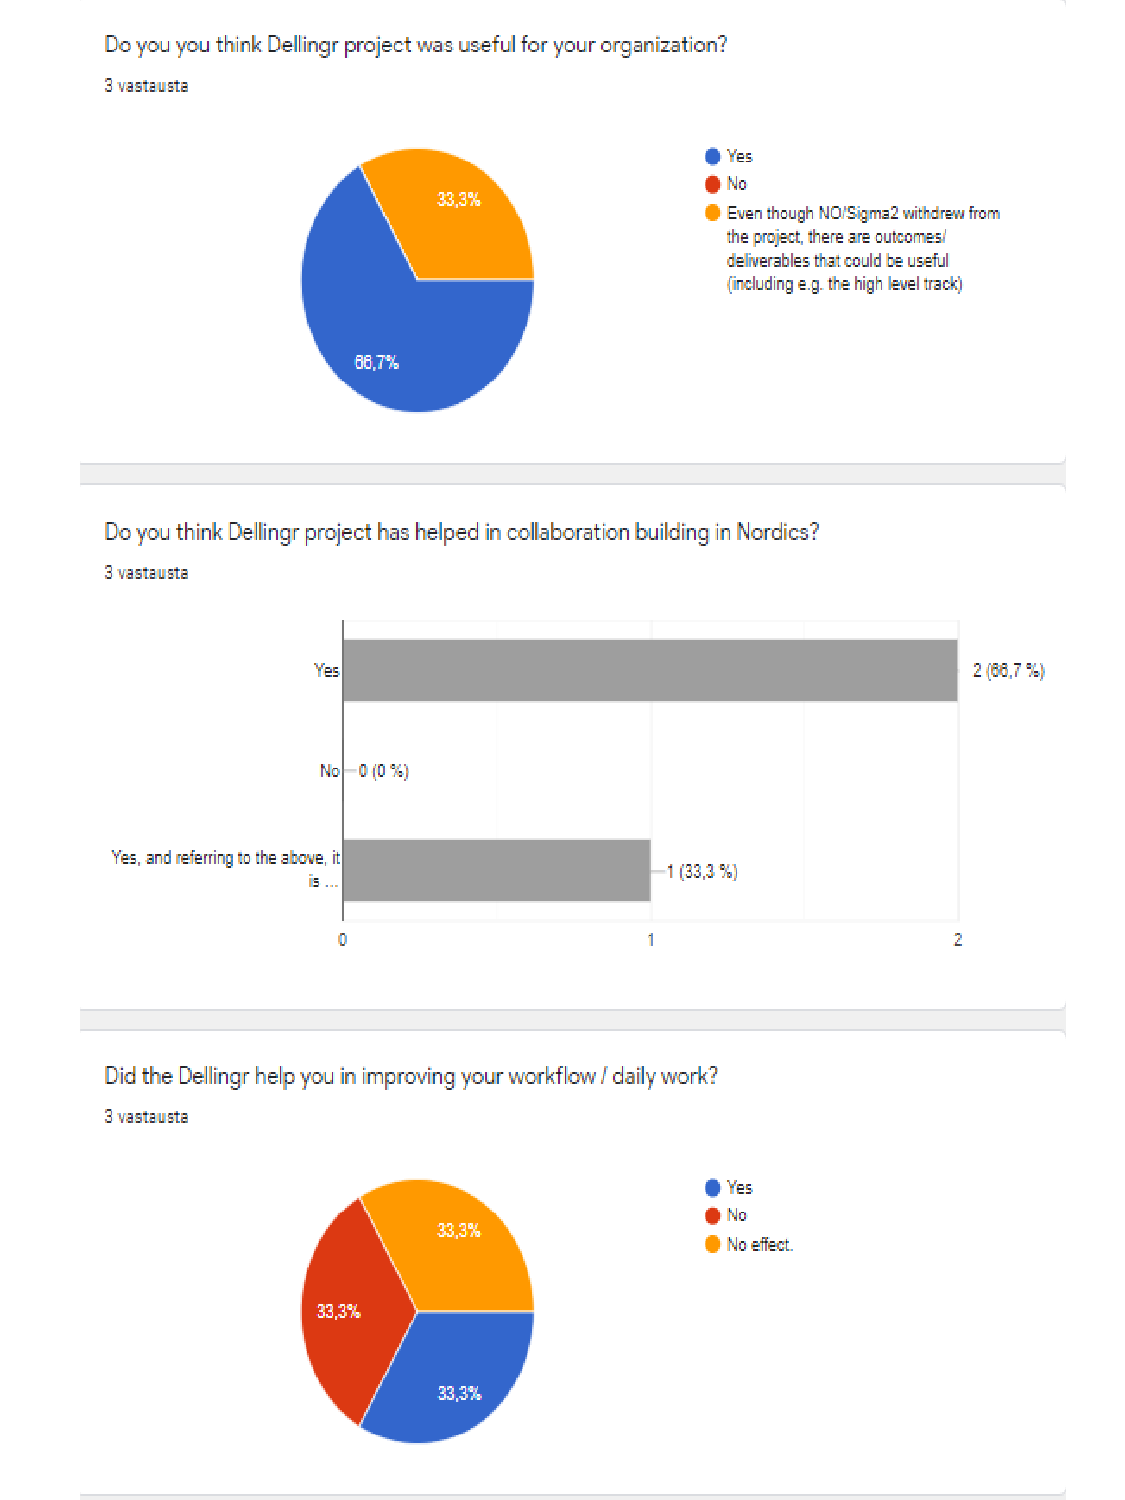
\includegraphics[scale=0.7]{SG_responses_1.pdf}
\end{center}

\begin{center}
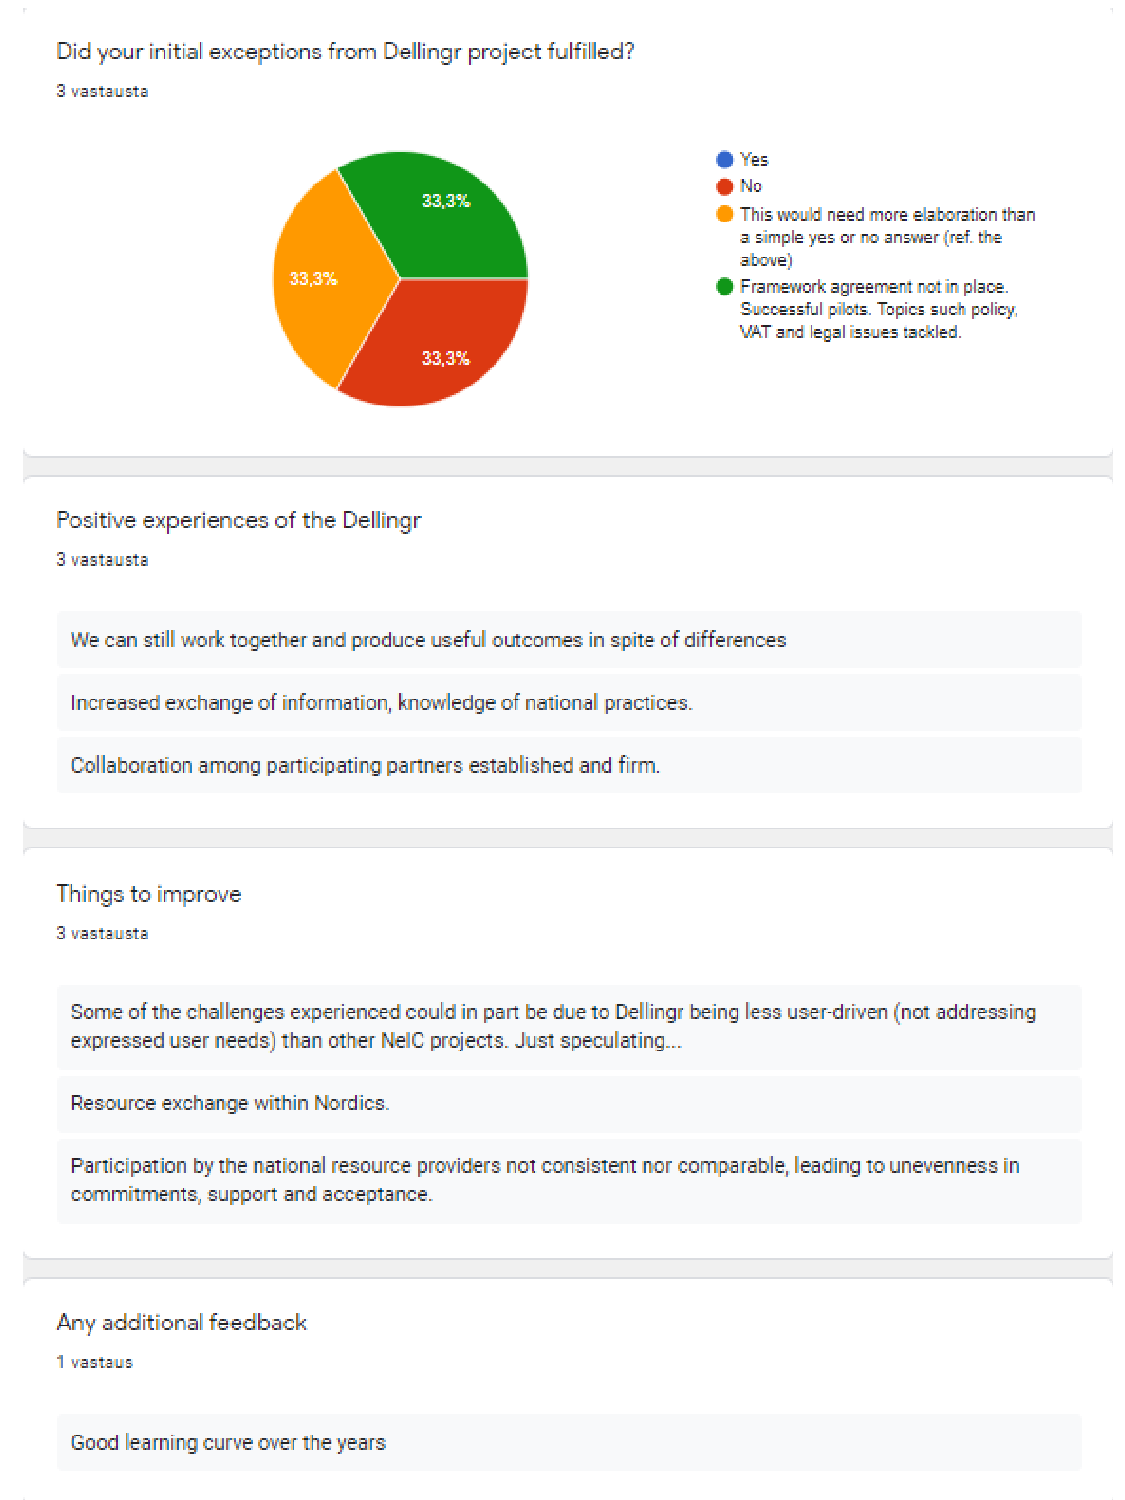
\includegraphics[scale=0.7]{SG_responses_2.pdf}
\end{center}

\section{\HLT Survey Responses}
\label{app:hlt-resp}

\begin{center}
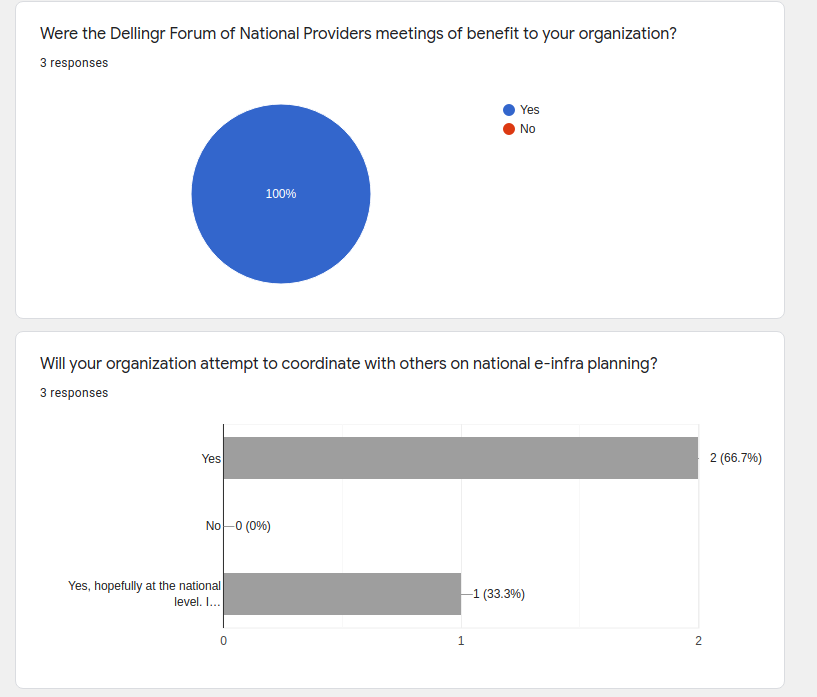
\includegraphics[scale=0.6]{hlt_responses_1.png}
\end{center}

\begin{center}
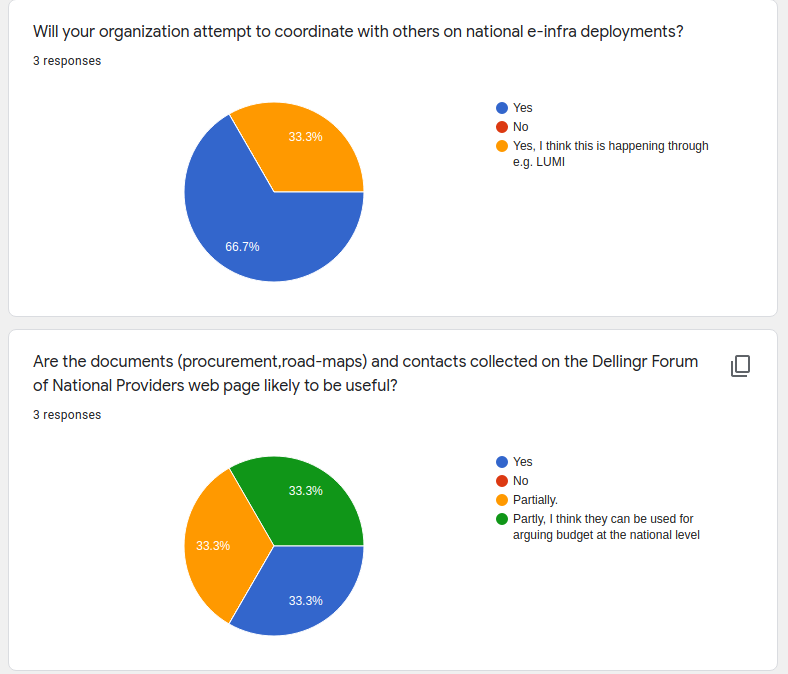
\includegraphics[scale=0.6]{hlt_responses_2.png}
\end{center}

\begin{center}
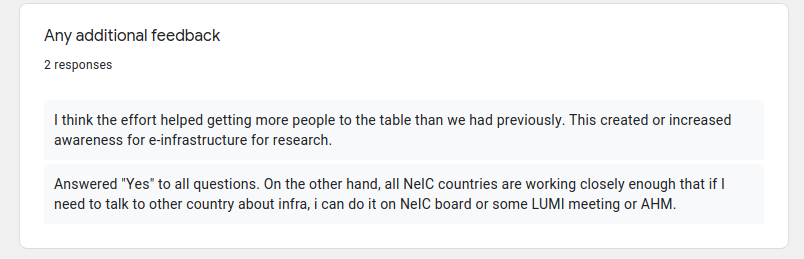
\includegraphics[scale=0.6]{hlt_responses_3.png}
\end{center}

\end{appendices}

\end{document}
